\documentclass[fullpage, 10pt, onecolumn, draftclsnofoot]{IEEEtran}
\usepackage[utf8]{inputenc}
\usepackage[margin=.75in]{geometry}
\usepackage{setspace}
%\usepackage{pgfgantt}
\usepackage{tabularx}
\usepackage{longtable}
\usepackage{amsmath,amsthm,amssymb,amsfonts}
\usepackage{graphicx}
\usepackage{float}
\usepackage{multirow}
\usepackage{url}
\usepackage{listings}
\usepackage{longtable}
\usepackage{tabularx}
\usepackage{xcolor}
\usepackage{setspace}
%\usepackage{pgfgantt}
\usepackage{caption}

\geometry{textheight=9.5in, textwidth=7in}
\lstdefinestyle{sharpc}{language=[Sharp]C, frame=lr, rulecolor=\color{blue!80!black}}
% Title Page Source: http://eecs.oregonstate.edu/capstone/cs/capstone.tex

% 1. Fill in these details
\def \CapstoneTeamName{WE SHOULD HAVE A TEAM NAME???}
\def \CapstoneTeamNumber{		66b}
\def \GroupMemberOne{			Austin Wilmoth}
\def \GroupMemberTwo{			Bao Phung}
\def \GroupMemberThree{			Harry Miller}
\def \GroupMemberFour{			Justin Parks}
\def \GroupMemberFive{			Sonica Gupta}
\def \CapstoneProjectName{		Software Innovation for  Dual Screen Notebook}
\def \CapstoneSponsorCompany{	Intel}
\def \CapstoneSponsorPerson{		Mike Premi}

% 2. Uncomment the appropriate line below so that the document type works
\def \DocType{		%Problem Statement
				%Requirements Document
				%Technology Review
				% Design Document
				Winter End-Of-Term Report
				}
			
\newcommand{\NameSigPair}[1]{\par
\makebox[2.75in][r]{#1} \hfil 	\makebox[3.25in]{\makebox[2.25in]{\hrulefill} \hfill		\makebox[.75in]{\hrulefill}}
\par\vspace{-12pt} \textit{\tiny\noindent
\makebox[2.75in]{} \hfil		\makebox[3.25in]{\makebox[2.25in][r]{Signature} \hfill	\makebox[.75in][r]{Date}}}}
% 3. If the document is not to be signed, uncomment the RENEWcommand below
\renewcommand{\NameSigPair}[1]{#1}

%%%%%%%%%%%%%%%%%%%%%%%%%%%%%%%%%%%%%%%
\begin{document}


\begin{titlepage}
%    \pagenumbering{gobble}
    \begin{singlespace}
        \hfill 
        % 4. If you have a logo, use this includegraphics command to put it on the coversheet.
        %\includegraphics[height=4cm]{CompanyLogo}   
        \par\vspace{.2in}
        \centering
        \scshape{
            \huge Senior Capstone \DocType \par
            {\large March 17, 2020}\par
            \vspace{.5in}
            \textbf{\Huge\CapstoneProjectName}\par
            \vfill
            \huge Oregon State University \par
            \huge CS 462, Winter 2020 \par
            \vspace{.5in}
            {\large Prepared for}\par
            \Huge \CapstoneSponsorCompany\par
            \vspace{5pt}
            {\Large\NameSigPair{\CapstoneSponsorPerson}\par}
            {\large Prepared by }\par
            Group\CapstoneTeamNumber\par
            % 5. comment out the line below this one if you do not wish to name your team
% TEAM NAME ANYONE?? -->    %\CapstoneTeamName\par 
            \vspace{5pt}
            {\Large
                \NameSigPair{\GroupMemberOne}\par
                \NameSigPair{\GroupMemberTwo}\par
                \NameSigPair{\GroupMemberThree}\par
                \NameSigPair{\GroupMemberFour}\par
                \NameSigPair{\GroupMemberFive}\par
            }
            \vspace{20pt}
        }
        \begin{abstract}
        % 6. Fill in your abstract    


%An attempt to update the Abstract to cover the main sections of our paper

Our group will be building an application whose main function is to provide an easy setup for users who may use the notebook for a variety of purposes, such as music production, coding/productivity, and gaming/streaming. To provide tools to music producers, we will provide integration with a DAW, which requires programmable keyboard shortcuts and the ability to read and create virtual MIDI connections. For coding and productivity, user tests will give us insight in areas that would benefit those types of users on top of programmable hotkeys and auto-placement of windows.  The final use case, gaming/streaming, will be modeled on the UI of the Elgato Streamdeck, with the programmable buttons acting as quick access keys.
        \end{abstract}     
    \end{singlespace}
\end{titlepage}
\newpage

\singlespacing


\tableofcontents
\newpage
 
\section{Purpose}
Starting out, our purpose in this project was to create an application that would give people a reason to considering buying
a companion-screen notebook. Fast-forward a term and that is still our primary goal, but now we know the applications
that we will be creating, how we will go about creating them, and have a functional prototype that we can start testing. As of now, we would like our end-product to function,
in a broad-sense, similar to the Elgato Streamdeck - where users have programmable buttons that they can do a variety of
tasks with. \\ 
\newline
\indent Each member of the group was tasked with implementing part of the functionality of this application, with
some members taking specific use cases and others working on general quality of life aspects that will make the app more
usable. This includes a programming use case where a user might want keys to be able to auto-place multiple windows
and applications in a custom arrangement. A music production use case which will focus on integration with a DAW to let
the user be more productive in music creation. Along with many small issues we will have to solve like returning focus to
whichever application was currently taking focus before using this application and setting up UXs that are conductive to
actual user productivity increases.
\section{Goals}
The goal of this application is to help streamline the various tasks that the user needs to accomplish in order to boost productivity. We did this by binding applications and tasks to buttons in order to allow the user to do more in one step. Additionally, these buttons are then bound to keys so that the user is not only limited to pushing the button, but they also have the opportunity to just use keystrokes to accomplish their tasks. From there, this application is then scale-able to accomplish the specific tasks based on the user. For instance, a gamer might set up the application so that their moves and layouts are bound to different buttons and keystrokes. In this way, we are also able to take advantage of the companion screen so that the user is allowed an easy access to this grid of buttons.
% Describe where we are currently in the project
% describe what you have left to do
\section{Project State}
Our application takes the form of a widget so that upon booting the laptop, the application would appear in the companion screen, ready to use. There were a couple components of the application that we divided between ourselves which are going to be described in the following sections: design, auto focus, and a gaming use case.
\subsection{Design}
The goal for the layout of the application was to make so that the design is intuitive and easy to use. The Elgato Streamdeck featured buttons on the display that bound to the actions that the user wished. We used that same concept in our layout while also adding additional features to allow for both customization and scalability. We want to it to be customizable so that the users are able to use this application on the companion screen in a format that they find visually appealing. We also wanted this application to be scalable as there are so many use cases (streaming, production, programming, etc) for this application that the user should be able to set it up as they wish to. \\
\newline
\indent Ideally, when the user starts their laptop, this application will be ready to go for them. Thus, upon the first boot of the application, before the user has a chance to customize the grid, the only thing visible to the user would be the top navigation bar, as shown in Figure 1. Otherwise, once the user has customized it, they would see all their buttons on the grid.

\begin{figure}[H]
    \centering
    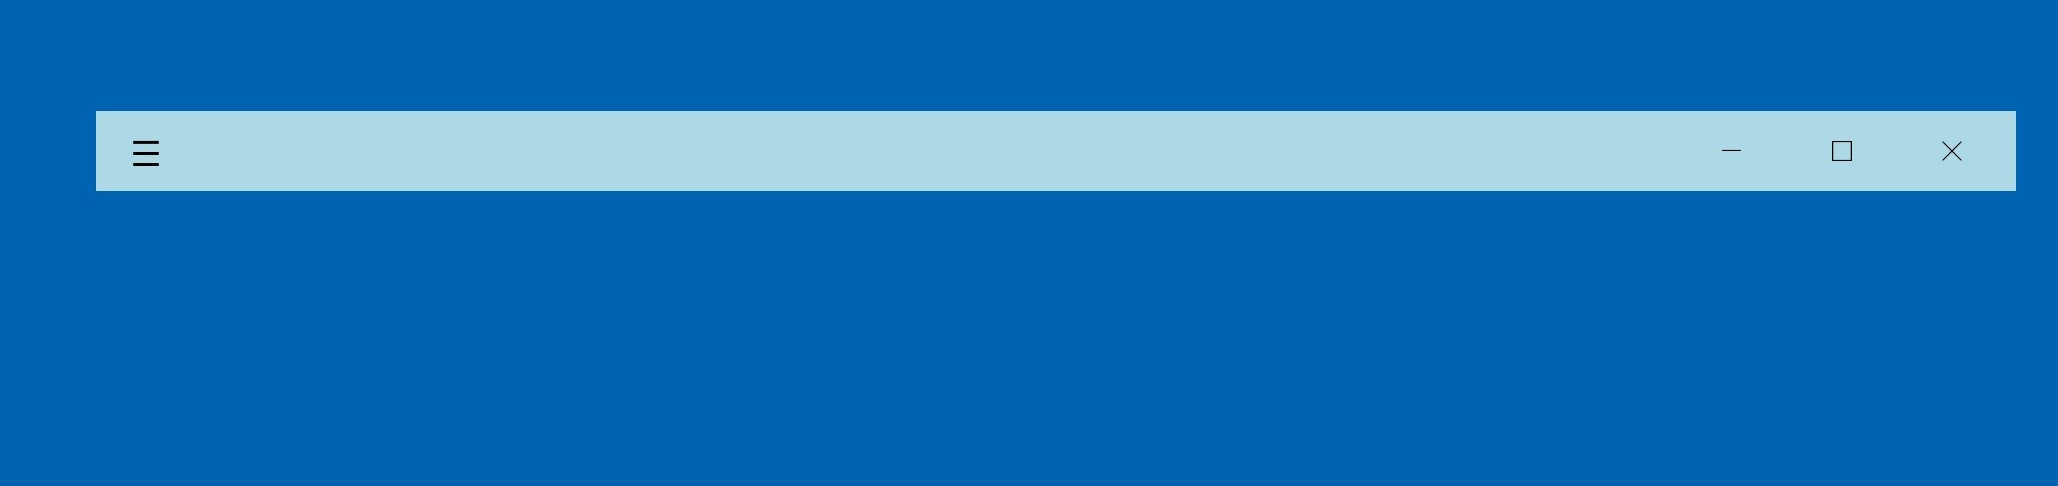
\includegraphics[width=14cm, height=4cm]{images/topBar.jpg}
    \caption{Top Bar}
    \label{fig:my_label}
\end{figure}

From there, the user would be able to interact with the application through the navigation drawer, pictured in the top left of Fig 1, and come to a layout similar to: 
\begin{figure}[H]
    \centering
    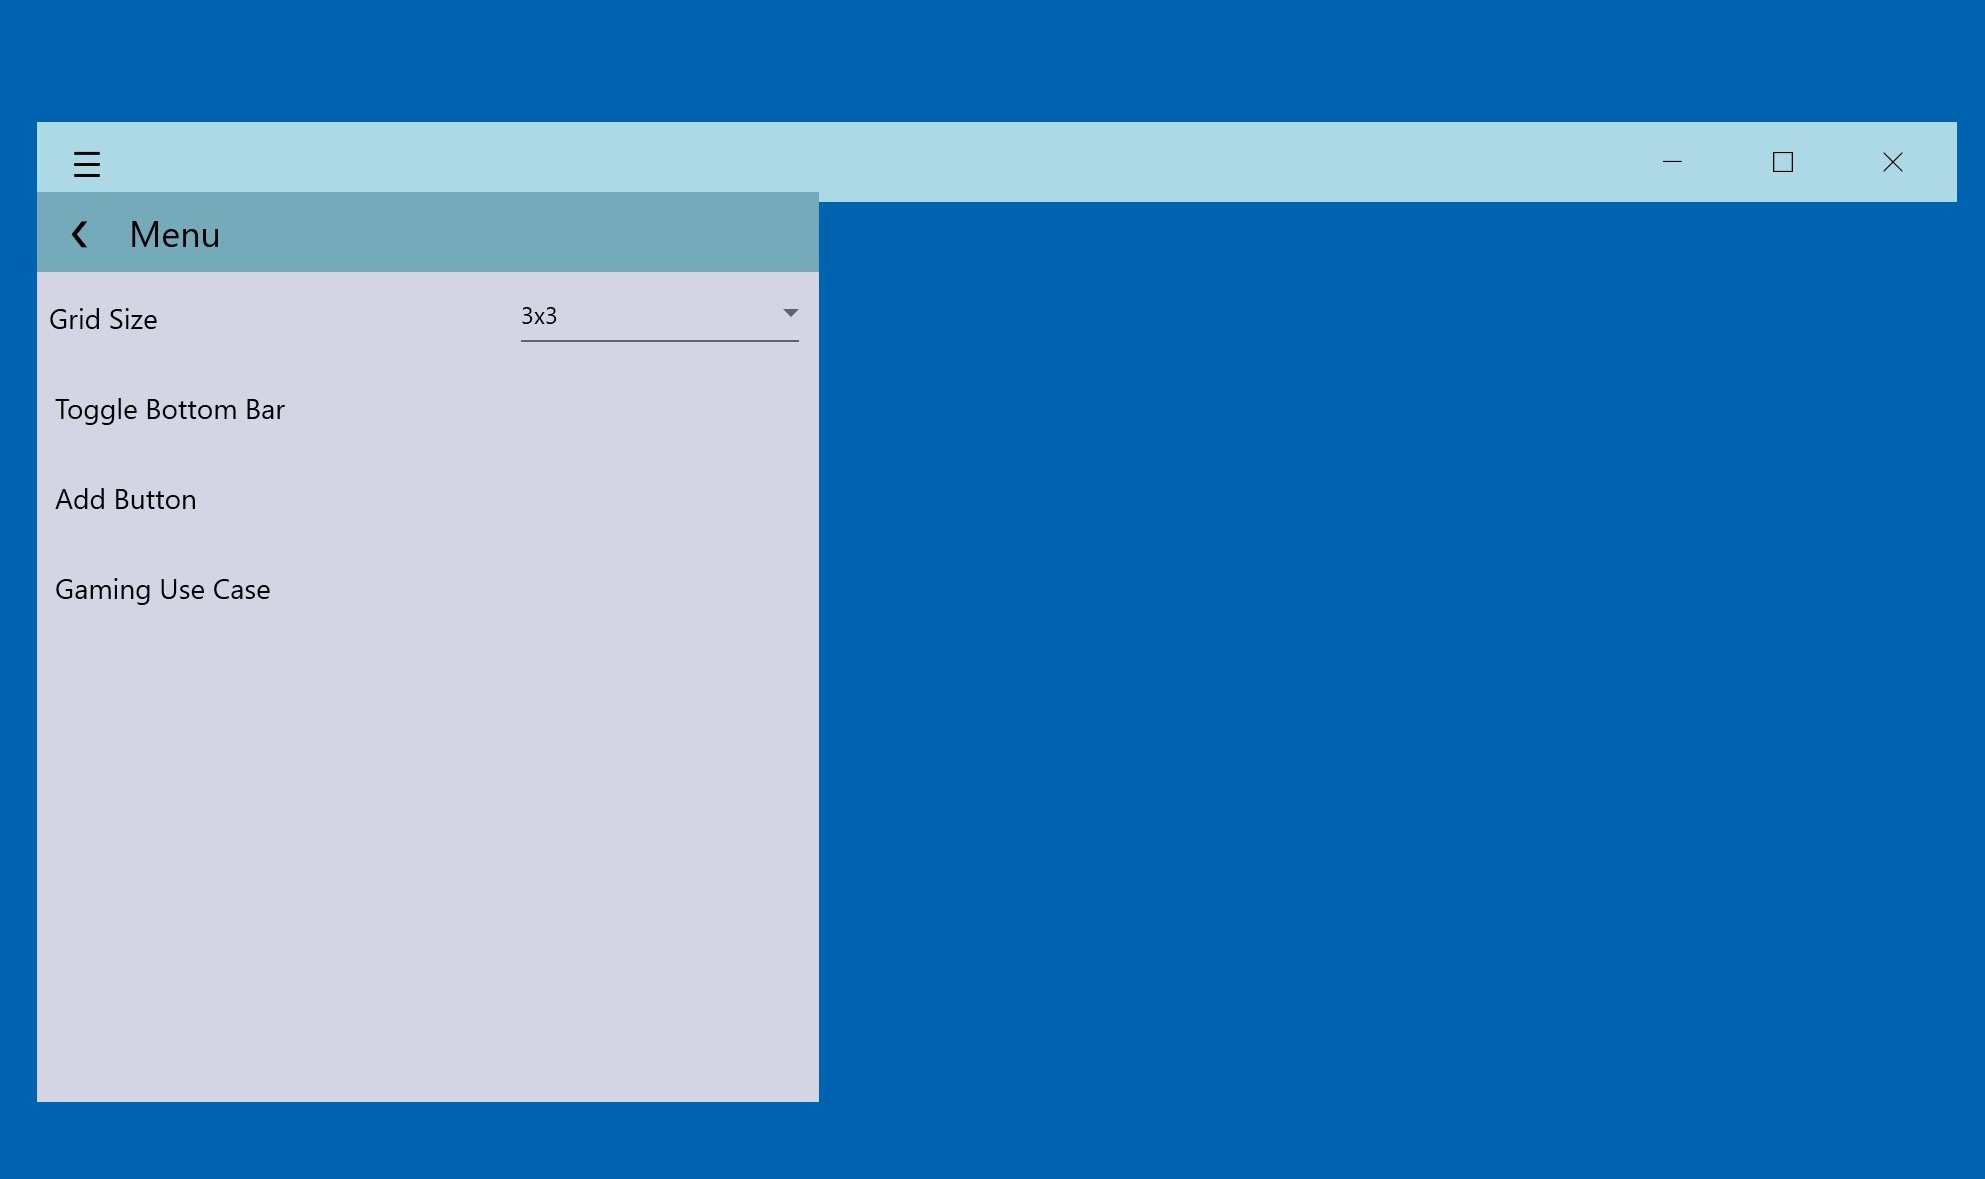
\includegraphics[width=14cm, height=8cm]{images/navBar.jpg}
    \caption{Menu}
    \label{fig:my_label}
\end{figure}
Here, in the navigation drawer, the user is able to do a couple different things.
\begin{itemize}
    \item Grid Size: Here, the user is able to change the dimensions of the buttons. For instance, if they wanted a 3x3 grid, 1x4 grid, etc. Depending on how many buttons their task requires, they can adjust the dimensions. Figure 3 below shows the dimensions that come preset with the application.  
    \begin{figure}[H]
        \centering
        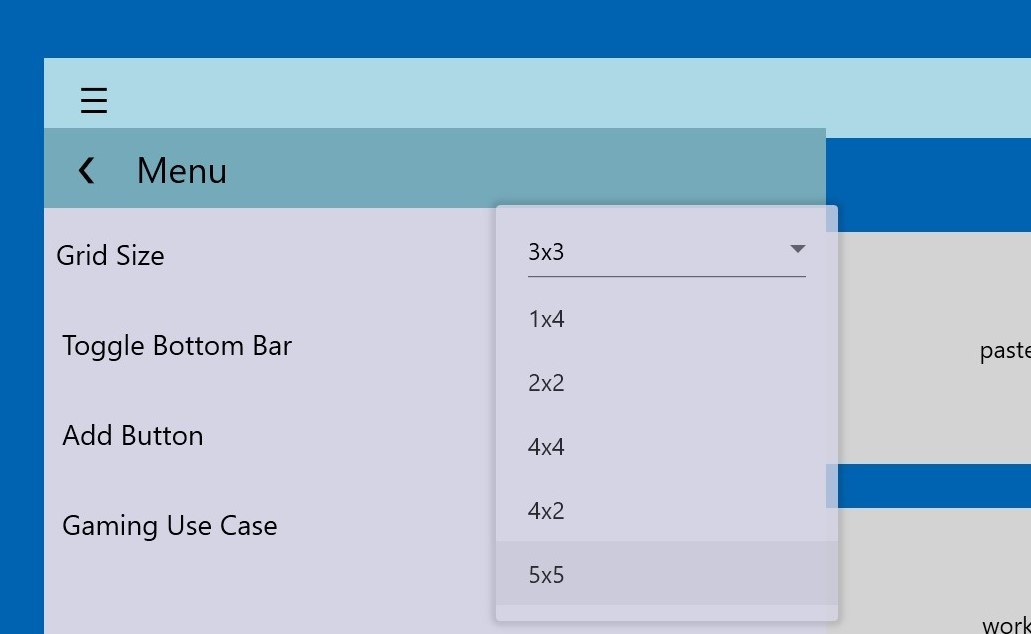
\includegraphics[width=7cm, height=4cm]{images/grid.jpg}
        \caption{Optional Grid Dimensions}
        \label{fig:my_label}
    \end{figure}
    \item Toggle Bottom Bar: This button allows you to add or remove the bottom bar. The bottom bar is used as a media control, pictured in Figure 4 below. On the left, the user has its normal media controls, play/pause, forward, and rewind that will work with whatever media is playing. On the right, there are undo and redo options to help the user undo or redo their last actions. This is helpful if the user wants to undo an action or redo an action. 
    \begin{figure}[H]
        \centering
        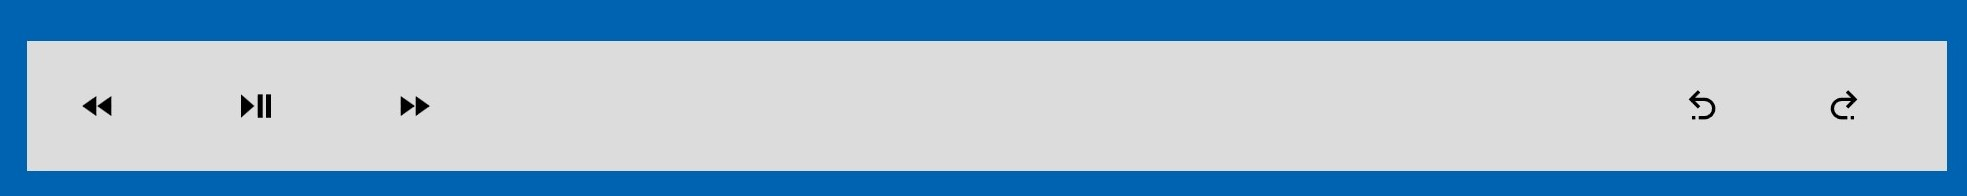
\includegraphics[width=14cm, height=2cm]{images/BottomBar.jpg}
        \caption{Media Bar}
        \label{fig:my_label}
    \end{figure}
    \item Add Button: This menu is used if the user wants to add a shortcut or a button to their grid. The first field prompts the user for a shortcut name, which would just be the name of the button that the user is creating. The second field allows the user to add application(s) to launch on click of the button. The user could either give the path to file, give the executable name, or search for the file that they want using the file browser on the right. The last field prompts the user for a keyboard shortcut. This makes it so that the user does not need to keep clicking on the buttons but could instead launch the task through keystrokes. 
    \begin{figure}[H]
        \centering
        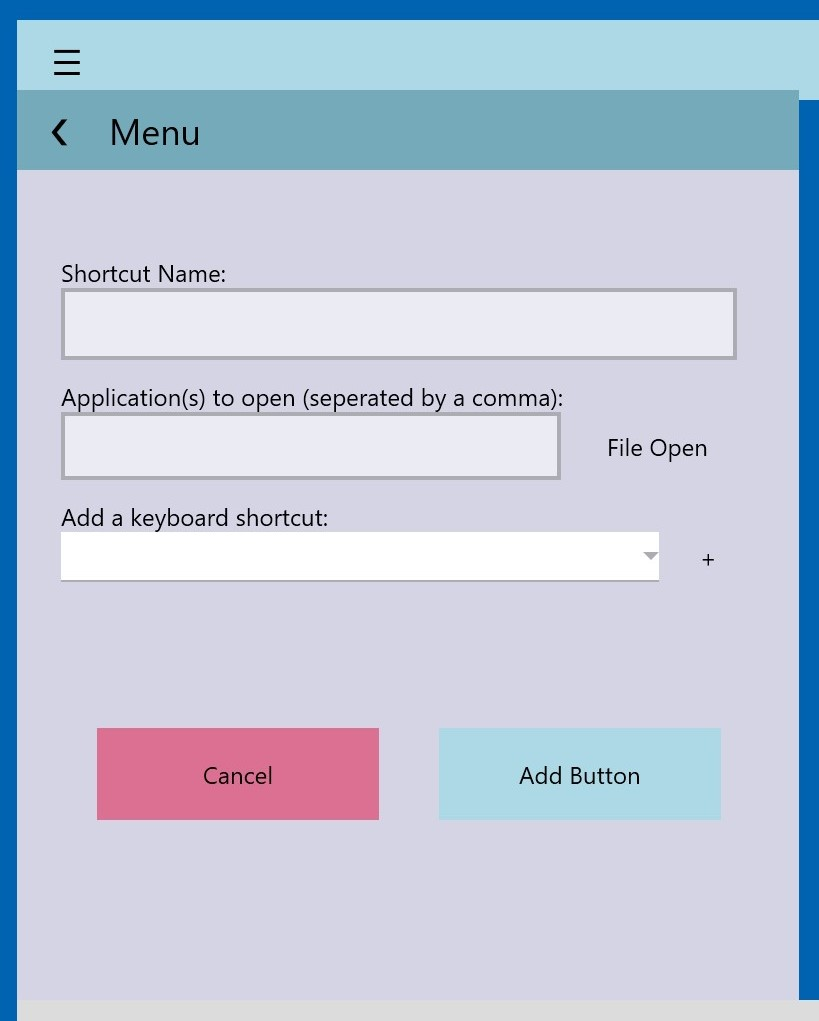
\includegraphics[width=6cm, height=7cm]{images/addButtonMenu.jpg}
        \caption{Add Button Menu}
        \captionsetup{justification=centering}
        \label{fig:my_label}
    \end{figure}
    \item{Gaming Use Case:} This button corresponds to one of the preset use cases that we created. The buttons corresponds to different games that could booted and different move that could be used within the games. More on this is described in Section C.\\  
\end{itemize}
Coming together, an instance of this application could look like the image in Figure 6. The buttons are laid out in a 3x3 grid overlaid a transparent background. The buttons could either be clicked to perform the action or the user could use the keystrokes that bound to the buttons to perform the actions. The users also have the option of moving the buttons around by either holding down on the button or left-clicking it. 
\begin{figure}[H]
    \centering
    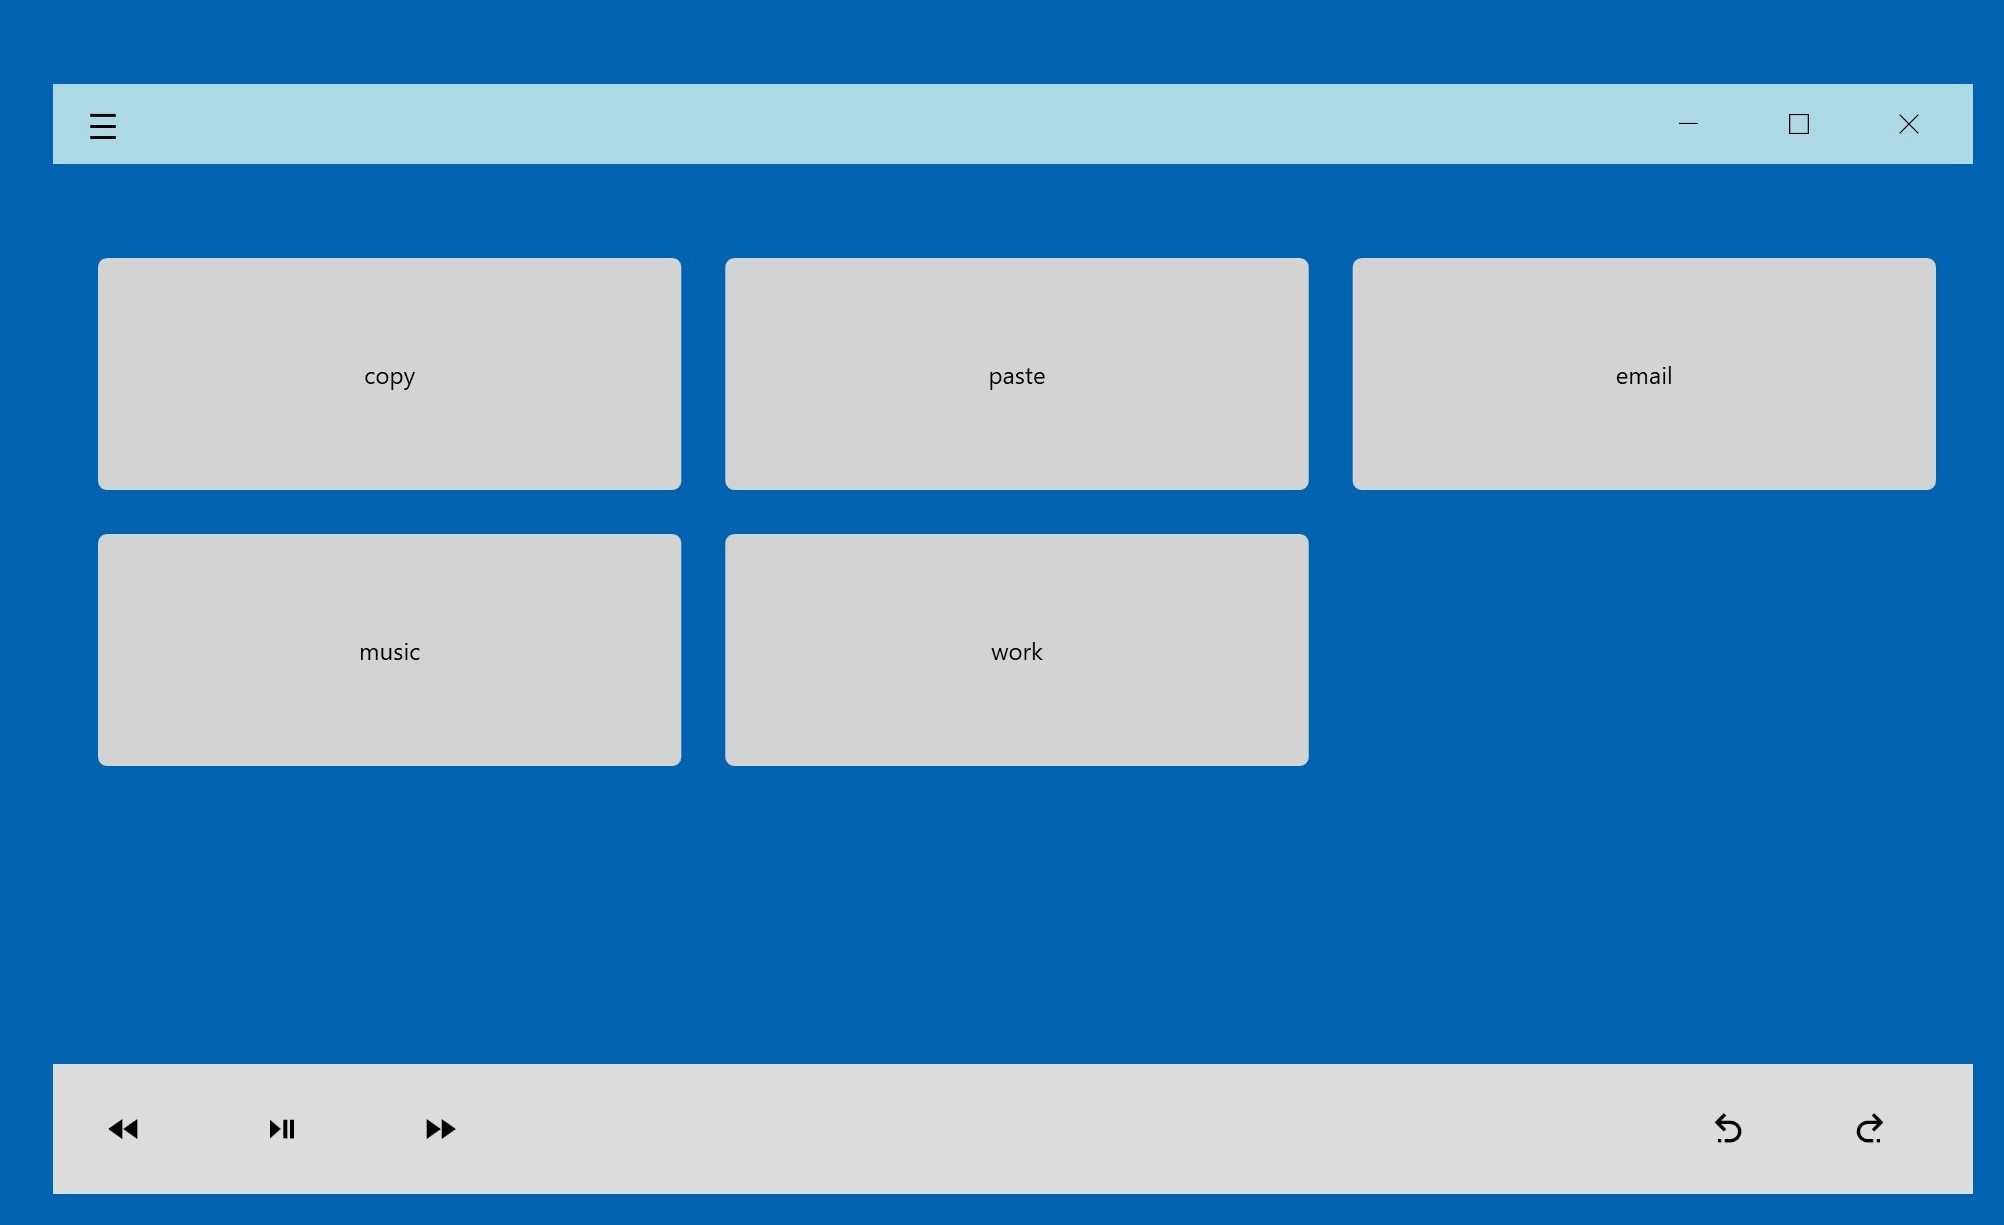
\includegraphics[height=7cm, width=14cm]{images/wButtons.jpg}
    \caption{Buttons in Application}
    \label{fig:my_label}
\end{figure}
\subsection{Returning Focus}
One issue that can easily become a problem when using a second screen is clicking something in the second app and then trying to use the original app again because the focus will have been changed to our application. We want, depending on the shortcut, to return the focus back to the application that the user is using.\\
\newline
\indent This was solved using windows APIs, specifically from the Winuser.h library. Using these APIs our application has the ability to set which application is in focus on the screen. This is done by setting the z-order of the window. What the z-order is is a value that represents what order each window is on the screen, the higher the z value the closer to focus the application is. This is how using alt-tab to change to another application on windows works. Each application further to the right is further on the z-axis and has a higher z value. For some applications, this won’t be too hard because the short cut will correspond to the application we want to go to. For example, if the user was using our program for programming they could click a shortcut that swapped what tab they were in in the IDE/text editor. This would put our app in focus and then we would send the focus right back to the previous app. For this, we will use the SetFocus which gives focus to the application that we tell it to.  \\
\newline
\indent This will work because we know exactly which application that the shortcut corresponds to. Other times it may be a bit more complected when the user clicks a shortcut that corresponds to another application than the one they had in focus before this will use a few more sets. For example while streaming a game the user clicks a short cut to mute their mic but they want to continue playing the game. In this case we have a few extra steps to get back to the application. A function that will be useful here is SetWindowPos. This lets the developer set the exact position that the application will be set. It is not just limited to the z value it can also set the x and y values as well, though not necessarily for solving this problem the x and y values will be useful for other aspects of our project. \\
\newline
\indent The following piece of code shows how this was made possible. The first part of the code is shown in the following snippet in a function called OnSourceInitialized. The problem that this snippet of code solves deals with the situation of when using two apps. For instance, if you need to need to do something on a side app, you will send a click, which would then take the focus away from your main app. In our case, we do not want the user to have to click on our application and have the focus take away from the their main application that they are currently using. In a case where they are using a game and want to send a keystroke, we do not want our application to take away focus.  \\
\newline
\indent One note on this code is that the line that sets window to WS\_EX\_NOACTIVE prevents the window from ever taking focus. This is helpful for us because then when we send an event to our application, the application will not take focus. \\
\newline
\lstset{style=sharpc}
\begin{lstlisting}
protected override void OnSourceInitialized(EventArgs e)
{
    base.OnSourceInitialized(e):
    shortcut = new List<VirtualKeyShort.Key>();
    helper = new WindowInteropHelper(this);
    SetWindowLong(helper.Handle, GWL_EXSTYLE, GetWindowLong(helper.Handle, 
        GWL_EXSTYLE) | WS_EX_NOACTIVE);
    HwndSource source = PresentationSource.FromVisual(this) as HwndSource;
    source.AddHook(WndProc);
    this.Activate();
}

\end{lstlisting} 

\noindent The previous function showed how our application did not take focus away from the other application that the user is using. However, this creates another issue that our application can not be interacted with at all because it is set to be not in focus. Thus, we now need to overwrite winproc. The following code snippet shows bow all the inputs in a window program was handled. Here, we force the click to still be handled, even if not in focus.
\lstset{style=sharpc}
\begin{lstlisting}
IntPrt WndProc(IntPtr hwnd, int msg, IntPtr wParam, IntPtr lParam, ref bool handled)
{
    switch (msg) 
    {
        case WM_MOUSEACTIVATE:
            return (IntPtr)MA_NOACTIVATE;
        default: 
            break;
    }
}
\end{lstlisting}




\subsection{Gaming Use Case}
As inspired by the Elgato Streamdeck, this use case allows for users to actually load/save any of their application configurations and open them with either an alphanumeric key press, a button click, or a touch (if the screen is touchable).  Essentially, within the menu as listed in Fig. 2, users are able to access the gaming use case application, which can be seen in Fig. 7 below.\\

\begin{figure}[H]
    \centering
    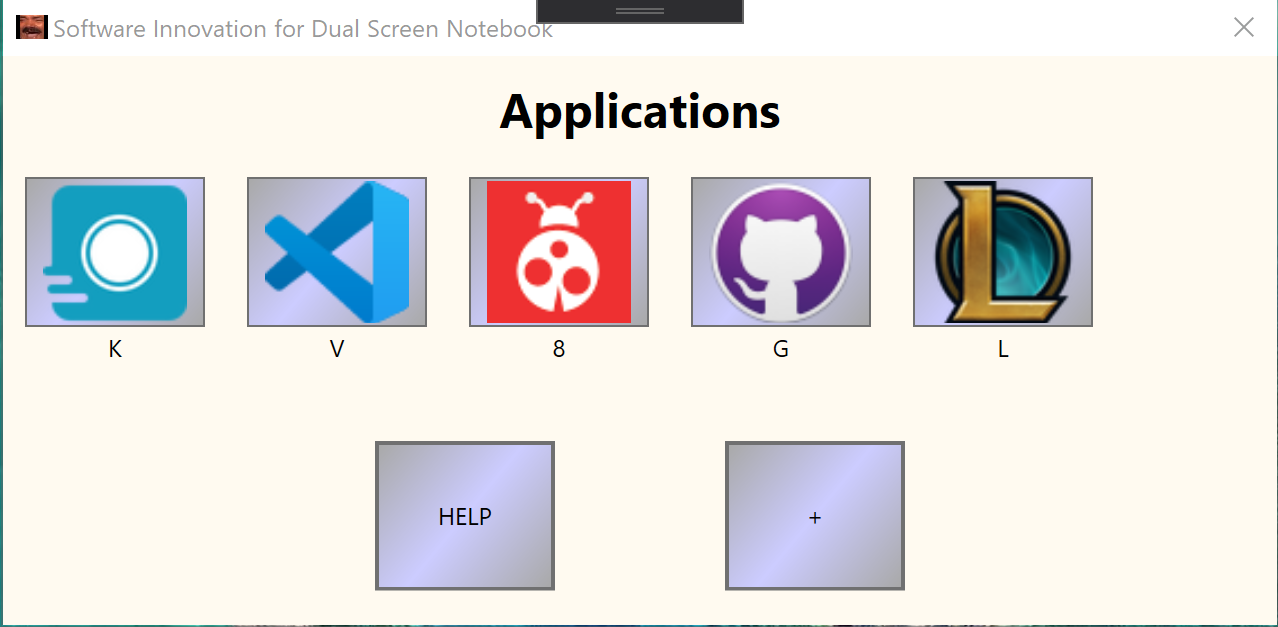
\includegraphics[height=7cm, width=14cm]{images/gamingHomeScreen.PNG}
    \caption{Home Screen of Gaming Use Case, with Preset Applications loaded}
    \label{fig:my_label}
\end{figure}

Looking at the layout, users have the option of opening any one of the five applications with either pressing their respective alphanumeric keys, clicking on the button corresponding to the application, or simply touching the button if the user's computer supports touch screen.  In addition, there are two additional buttons that corresponding to popping up a help form and an Add Application form, respectively.  The help form simply opens a pop up that instructs each user how to use this application.  The add form opens a form that takes 3 inputs: a required application that is retrieved from the user's computer, a nonrequired image if the user wants the application to have a custom image on the Gaming Use case, and a required hotkey that is alphanumeric and is unique - and also does not differentiate between uppercase and lowercase letters.  Fig. 7 does not show it, but there is also a scrollable option, but only if the number of buttons exceed the current space of the width layout. \\

One last feature of the gaming use case is the ability to save and load configurations and layouts.  Because the layouts and configurations are saved only for this specific use case, the following code snippet below depicts the logic necessary to accomplish this task.\\

\lstset{style=sharpc}
\begin{lstlisting}
while ((application = reader.ReadLine()) != null)
    {
        //4 lines per application:
        /*
         *  1. Application name
         *  2. Button height, width, and margins 
         *  3. Image location (unless n), height, width, and transformation origins
         *  4. Text margins
         */

        //If we encounter an empty string, stop
        if (application == "")
            break;

        // For steps 2-4, we need a tokenizer
        char[] separator = { ' ' };

        // Step 2 (requires tokenizing)
        string[] buttonInfo = reader.ReadLine().Split(separator);
        int buttonHeight = Int32.Parse(buttonInfo[0]);
        int buttonWidth = Int32.Parse(buttonInfo[1]);
        int buttonMarginOne = Int32.Parse(buttonInfo[2]);
        int buttonMarginTwo = Int32.Parse(buttonInfo[3]);

        // Step 3 (requires tokenizing)
        string[] imageInfo = reader.ReadLine().Split(separator);
        string imageLocation = imageInfo[0];
        if (imageLocation == "n")
            imageLocation = "";
        int imageHeight = Int32.Parse(imageInfo[1]);
        int imageWidth = Int32.Parse(imageInfo[2]);
        double originOne = Double.Parse(imageInfo[3]);
        double originTwo = Double.Parse(imageInfo[4]);

        // Step 4 (requires parsing)
        string[] textInfo = reader.ReadLine().Split(separator);
        int textMarginOne = Int32.Parse(textInfo[0]);
        int textMarginTwo = Int32.Parse(textInfo[1]);
        int textMarginThree = Int32.Parse(textInfo[2]);
        int textMarginFour = Int32.Parse(textInfo[3]);
        char hotkey = textInfo[4][0];

        // Then load that button dynamically
        AddApplication(application,
                    buttonHeight, buttonWidth, buttonMarginOne, buttonMarginTwo,
                    imageLocation, imageHeight, imageWidth, originOne, originTwo,
            textMarginOne, textMarginTwo, textMarginThree, textMarginFour, hotkey);
    }
\end{lstlisting} 

Essentially, this snippet of code reads from a file, where the file contains a list of applications.  Each application has four important lines as detailed in the comments.  The snippet basically extracts each line and then tokenizes, which we then take each tokenized part as an argument to the AddApplication function that is called last.


\section{Next Steps}
The remaining steps we want to complete are better defining specific use cases and letting the user save their settings (note that the gaming use case already accomplishes this task).  By defining use cases it would allow us to create more targeted and focused utilities that would attract niche communities to our application.  Saving user configurations is extremely necessary for our application because it would be overly tedious to have to recreate a user's setup upon closing the application, defeating it's intended purpose to save time.  The user interface has been improved since alpha functionality but we plan to do some user testing to receive feedback about any changes that could help with the user experience.  

% describe any problems that have impeded your progress, with any solutions you have
\section{Problems} 
    In the duration of our project, only a few issues had shown up, but they were issues that required a bit of critical thinking to overcome. Firstly, when looking to implement the refocusing behavior when using the app, it became apparent that Universal Windows Platform (UWP) was not sufficient. In order to have this desired behavior, we would need to change over to a win32 environment with a Windows Presentation Foundation (WPF) UI frontend.\\ %MAYBE ADD THE CODE SNIPPIT HERE? % 
    \newline
    \indent Additionally, because of the time constraints and the relative complexity of both the gaming and music production use cases, we had to scale those back to meet the deadline for basic functionality. Both of those use cases required special UI configurations, which is often the trickiest and most difficult to perfect part. The overall functionality of the app will still help greatly in those two areas of interest, but it will be through the regular grid-like UI that is implemented now.


\end{document}
